

\input{"C:/Users/spileggi/Google Drive/STAT 330/Lectures/SlideStyle.tex"}



\title[Lecture 17]{PROC SQL}
\author[Pileggi]{Shannon Pileggi}

\institute[STAT 330]{STAT 330}

\date{}


\begin{document}

\begin{frame}
\titlepage
\end{frame}

\begin{frame}
\frametitle{OUTLINE\qquad\qquad\qquad} \tableofcontents[hideallsubsections]
\end{frame}


%===========================================================================================================================
\section[Overview]{Overview}
%===========================================================================================================================
\subsection{}

\begin{frame}
\ft{PROC SQL}
\begin{tabular}{lccc}
\hline
Task & \ttt{PROC SQL} & \ttt{DATA} step & Other \ttt{PROCs} \\
\hline\hline
Print results        & \gc  & \rx & \gc  \\
Sort data            & \gc  & \rx  & \gc  \\
Summarize data       & \gc  & \yt  & \gc  \\
Combine data         & \gc  & \gc  & \rx  \\
Create new variables & \gc  & \gc  & \rx  \\
Subset data          & \gc  & \gc  & \yt  \\
Create new data set  & \gc  & \gc  & \yt  \\
\hline
\end{tabular}
\end{frame}

\begin{frame}[fragile]
\ft{Syntax}
\bmp{0.51\textwidth}
\begin{code}{.}
PROC SQL;
   CREATE TABLE \emph{table-name} AS
   SELECT \emph{column(s)}
   FROM \emph{table(s)} | \emph{view(s)}
   WHERE \emph{expression}
   GROUP BY \emph{column(s)}
   ORDER BY \emph{column(s)}
   ;
QUIT;
\end{code}
\emp
\bmp{0.01\textwidth} \hspace{0.05in} \emp
\bmp{0.5\textwidth}
\bi
\item clauses \ttb{must} be specified in this order
\item only the \ttt{SELECT} and \ttt{FROM} clauses are required, all other clauses are optional
\item only one semi-colon for all clauses
\item terminology:
\item[]
\begin{tabular}{ll}
\hline
 SQL & SAS \\
\hline \hline
 table & data set \\
 row & observation  \\
 column & variable  \\
\hline
\end{tabular}
\ei
\emp
\end{frame}

\begin{frame}
\ft{Explanations}
\bmp{0.15\textwidth} \hspace{0.05in}\emp
\bmp{0.9\textwidth}
\bi
\item[\ttt{PROC SQL}] calls sql procedure \vskip7pt
\item[\ttt{CREATE TABLE}] create new data set (in lieu of print) \vskip7pt
\item[\ttt{SELECT}] specifies the column(s) (variables) to be selected \vskip7pt
\item[\ttt{FROM}] specifies the table(s) (data sets) to be queried \vskip7pt
\item[\ttt{WHERE}] subsets the data based on a condition \vskip7pt
\item[\ttt{GROUP BY}] classifies the data into groups based on the specified column(s) \vskip7pt
\item[\ttt{ORDER BY}] sorts the resulting rows (observations) by the specified column(s) \vskip7pt
\item[\ttt{QUIT}] ends the sql procedure
\ei
\emp
\end{frame}

\begin{frame}
\ft{SAS vs SQL}
\resizebox{1.0\textwidth}{!}{
\begin{tabular}{lll}
\hline
\ttb{Function} & \ttb{SQL} & \ttb{SAS} \\
\hline \hline
Drop columns & SELECT & DROP \\
Rename column & AS & RENAME \\
Add rows & INSERT INTO & OUTPUT \\
Delete rows & DELETE FROM / WHERE & WHERE / IF-THEN / DELETE \\
Delete duplicate rows & DISTINCT & NODUPLICATE \\
Create a table & CREATE TABLE & DATA \\
Sorting & ORDER BY & PROC SORT \\
Summarize data & GROUP BY &  PROCs / FIRST. LAST. \\
Conditional statement & CASE-WHEN & IF-THEN \\
Displaying output & SELECT & PROC PRINT \\
Concatenating & OUTER JOIN & SET \\
\hline
\end{tabular}}
\end{frame}


%===========================================================================================================================
\section[SELECT]{SELECT}
%===========================================================================================================================
\subsection{}
\begin{frame}
\tableofcontents[currentsection, hideallsubsections]
\end{frame}


\begin{frame}[fragile]
\ft{Getting started with SELECT}
\bmp{.45\textwidth}
\begin{code}{.}
PROC SQL;
   SELECT \textcolor{OrangeRed}{*}
   FROM patents
   ;
QUIT;


PROC SQL;
   SELECT region\textcolor{OrangeRed}{,}
          division\textcolor{OrangeRed}{,}
          county\textcolor{OrangeRed}{,}
          patents
   FROM patents
   ;
QUIT;
\end{code}
\emp
%\bmp{.03\textwidth} \hspace{0.05in} \emp
\bmp{.50\textwidth}
\begin{itemize}
\item[]
\item \ttt{*} specifies \emph{all} variables
\item[]
\item indicate specific variables in a list separated by commas
\item[] 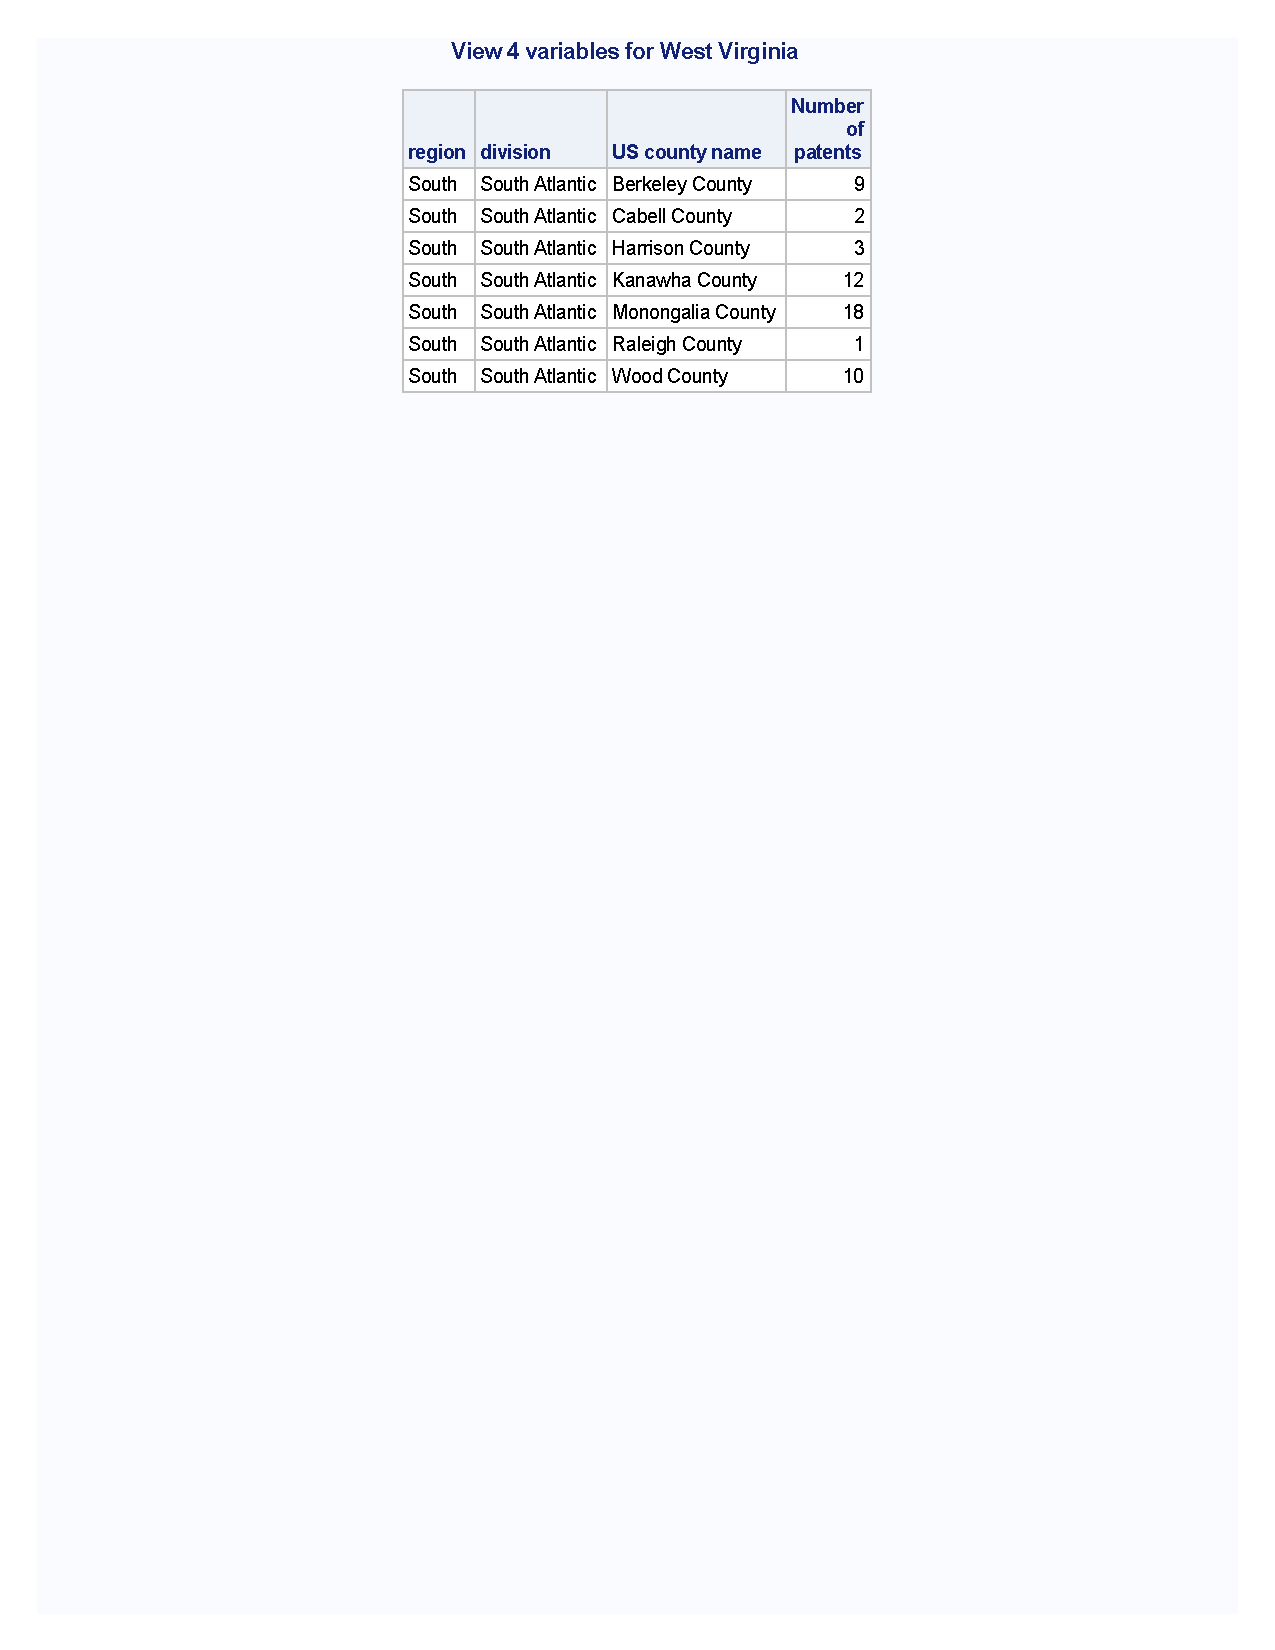
\includegraphics[trim={6.5cm 21cm 6.5cm 1.5cm},clip,width=1.0\textwidth]{L17_select.pdf}
\item[]
\end{itemize}
\emp
\end{frame}

\begin{frame}[fragile]
\ft{Calculating a new variable}
\hspace*{-0.3in}
\bmp{.66\textwidth}
\begin{code}{.}
PROC SQL ;
   SELECT  county, patents, population,
           \textcolor{OrangeRed}{(population/10000) AS pop10k}
   FROM patents
   WHERE state = "WEST VIRGINIA"
         AND \textcolor{OrangeRed}{calculated pop10k > 10}
	;
QUIT ;
\end{code}
\emp
\blankcolumn
\bmp{.40\textwidth}
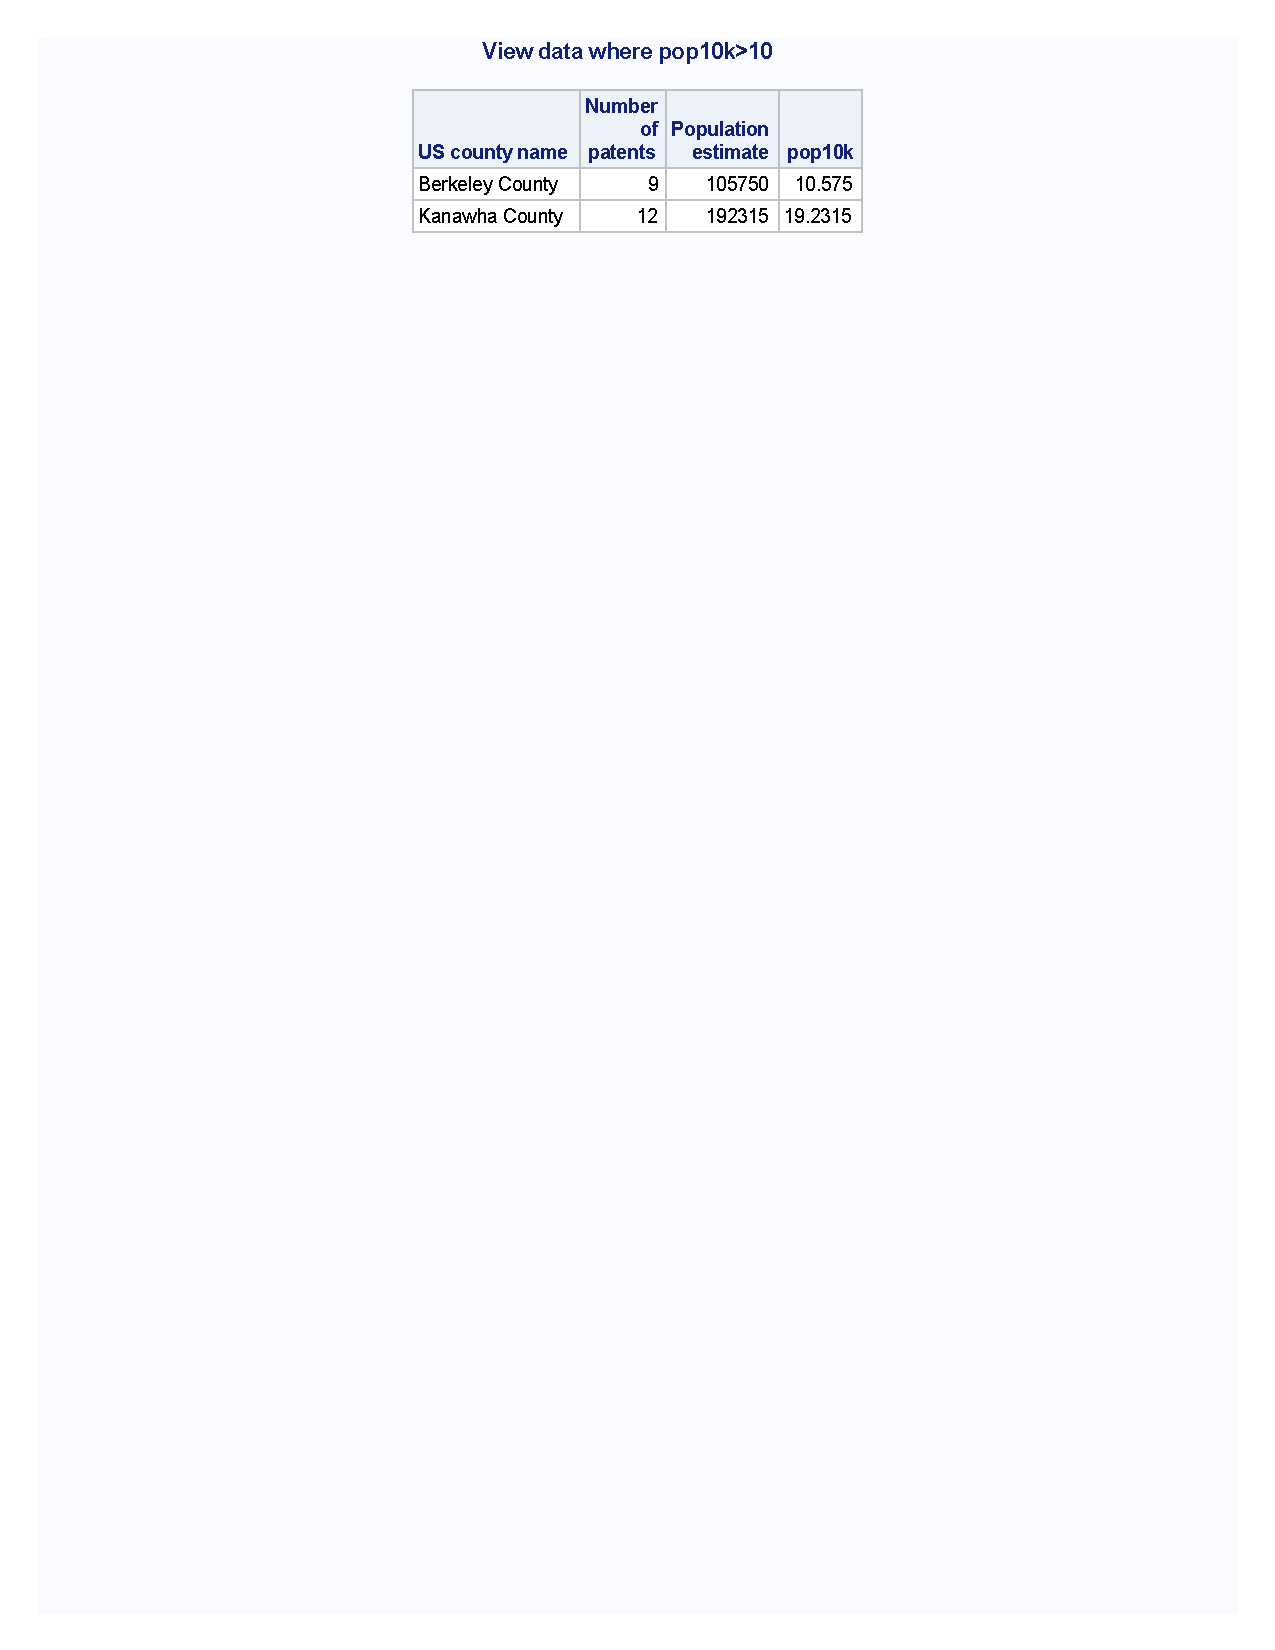
\includegraphics[trim={6.5cm 23cm 6.5cm 1.5cm},clip,width=1.0\textwidth]{L17_calculate.pdf}
\emp
\vskip5pt
\begin{itemize}
\item Syntax: \fbox{\ttt{(\emph{expression}) as \emph{newvar}}} \vskip5pt
\item When using \emph{newvar} in subsequent code, must refer to it as
\item[]\fbox{\ttt{calculated \emph{newvar}}}
\end{itemize}
\end{frame}

\begin{frame}[fragile]
\ft{Apply labels and formats}
\hspace*{-0.3in}
\bmp{1.1\textwidth}
\begin{code}{.}
PROC SQL ;
   SELECT region, division, county,
      patents \textcolor{OrangeRed}{LABEL = "Patents"},
      population \textcolor{OrangeRed}{FORMAT = COMMA15. LABEL = "Population"}
   FROM patents
   WHERE state = "WEST VIRGINIA"
   ;
QUIT;
\end{code}
\emp
\vskip5pt
\hspace*{-0.3in}
\bmp{0.70\textwidth}
\emph{after} variable name \emph{before} comma:
\begin{itemize}
\item apply format with \fbox{\ttt{format=\emph{myfmt.}}}
\item apply label with  \fbox{\ttt{label=\emph{"mylabel"}}}
\end{itemize}
\emp
%\blankcolumn
\bmp{0.45\textwidth}
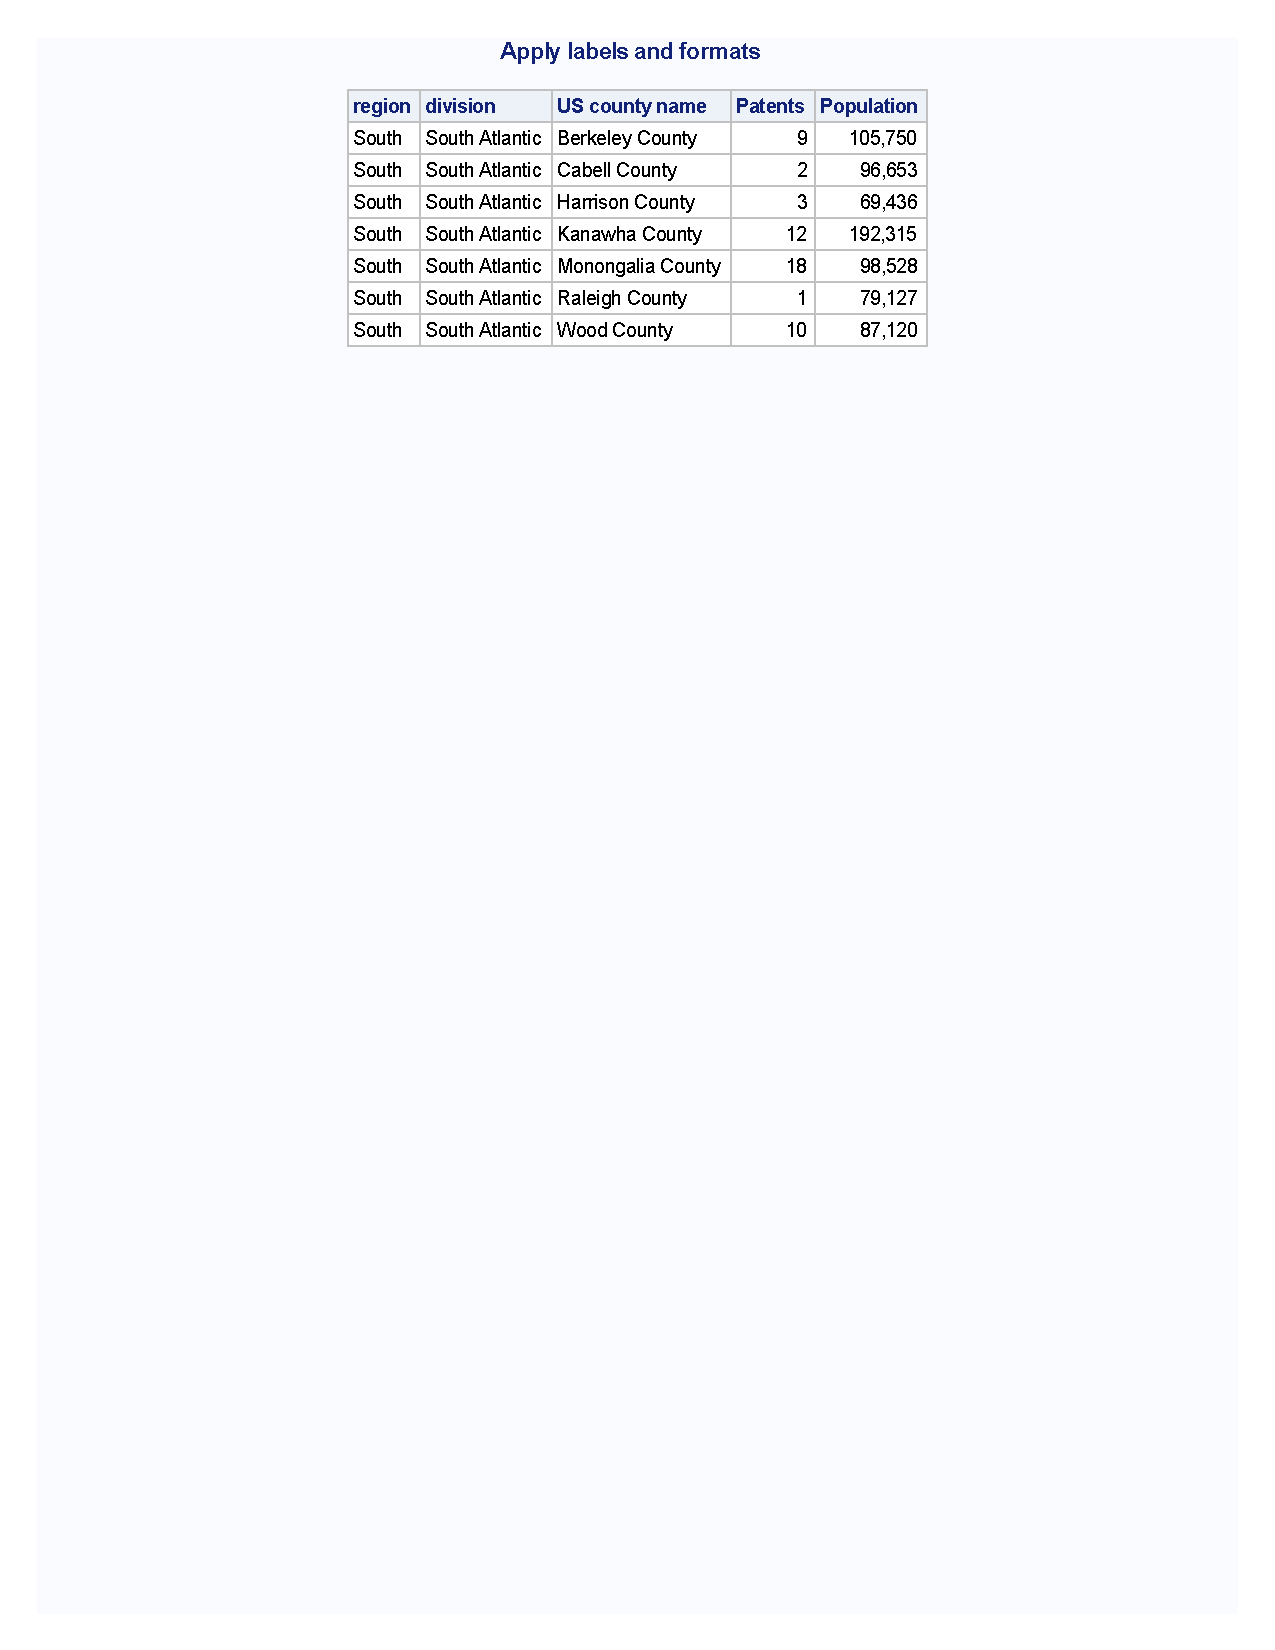
\includegraphics[trim={5.5cm 21cm 5.5cm 1.5cm},clip,width=1.0\textwidth]{L17_labelformat.pdf}
\emp
\end{frame}

\begin{frame}[fragile]
\ft{Creating a new variable with conditional logic}
\bmp{1.05\textwidth}
\begin{code}{.}
PROC SQL ;
   SELECT region, division, county, patents LABEL = "Patents",
   population FORMAT = COMMA15. LABEL = "Population",
   \textcolor{OrangeRed}{CASE}
      \textcolor{OrangeRed}{WHEN} population LE 70000 THEN "small"
      \textcolor{OrangeRed}{WHEN} population BETWEEN 70001 AND 120000 THEN "medium"
      \textcolor{OrangeRed}{ELSE} "large"
   \textcolor{OrangeRed}{END AS} size
   FROM patents ;
QUIT ;
\end{code}
\emp
\vskip5pt
\begin{itemize}
\item \ttt{CASE - WHEN/THEN/ELSE - END} similar to \ttt{IF-THEN-ELSE}
\item use \fbox{\ttt{END AS \emph{newvar}}} to create a new variable
\item when using \emph{newvar} in subsequent code, must refer to it as
\item[]\fbox{\ttt{CALCULATED \emph{newvar}}}
\end{itemize}
\end{frame}

\begin{frame}[fragile]
\ft{Creating a new variable with conditional logic, output}
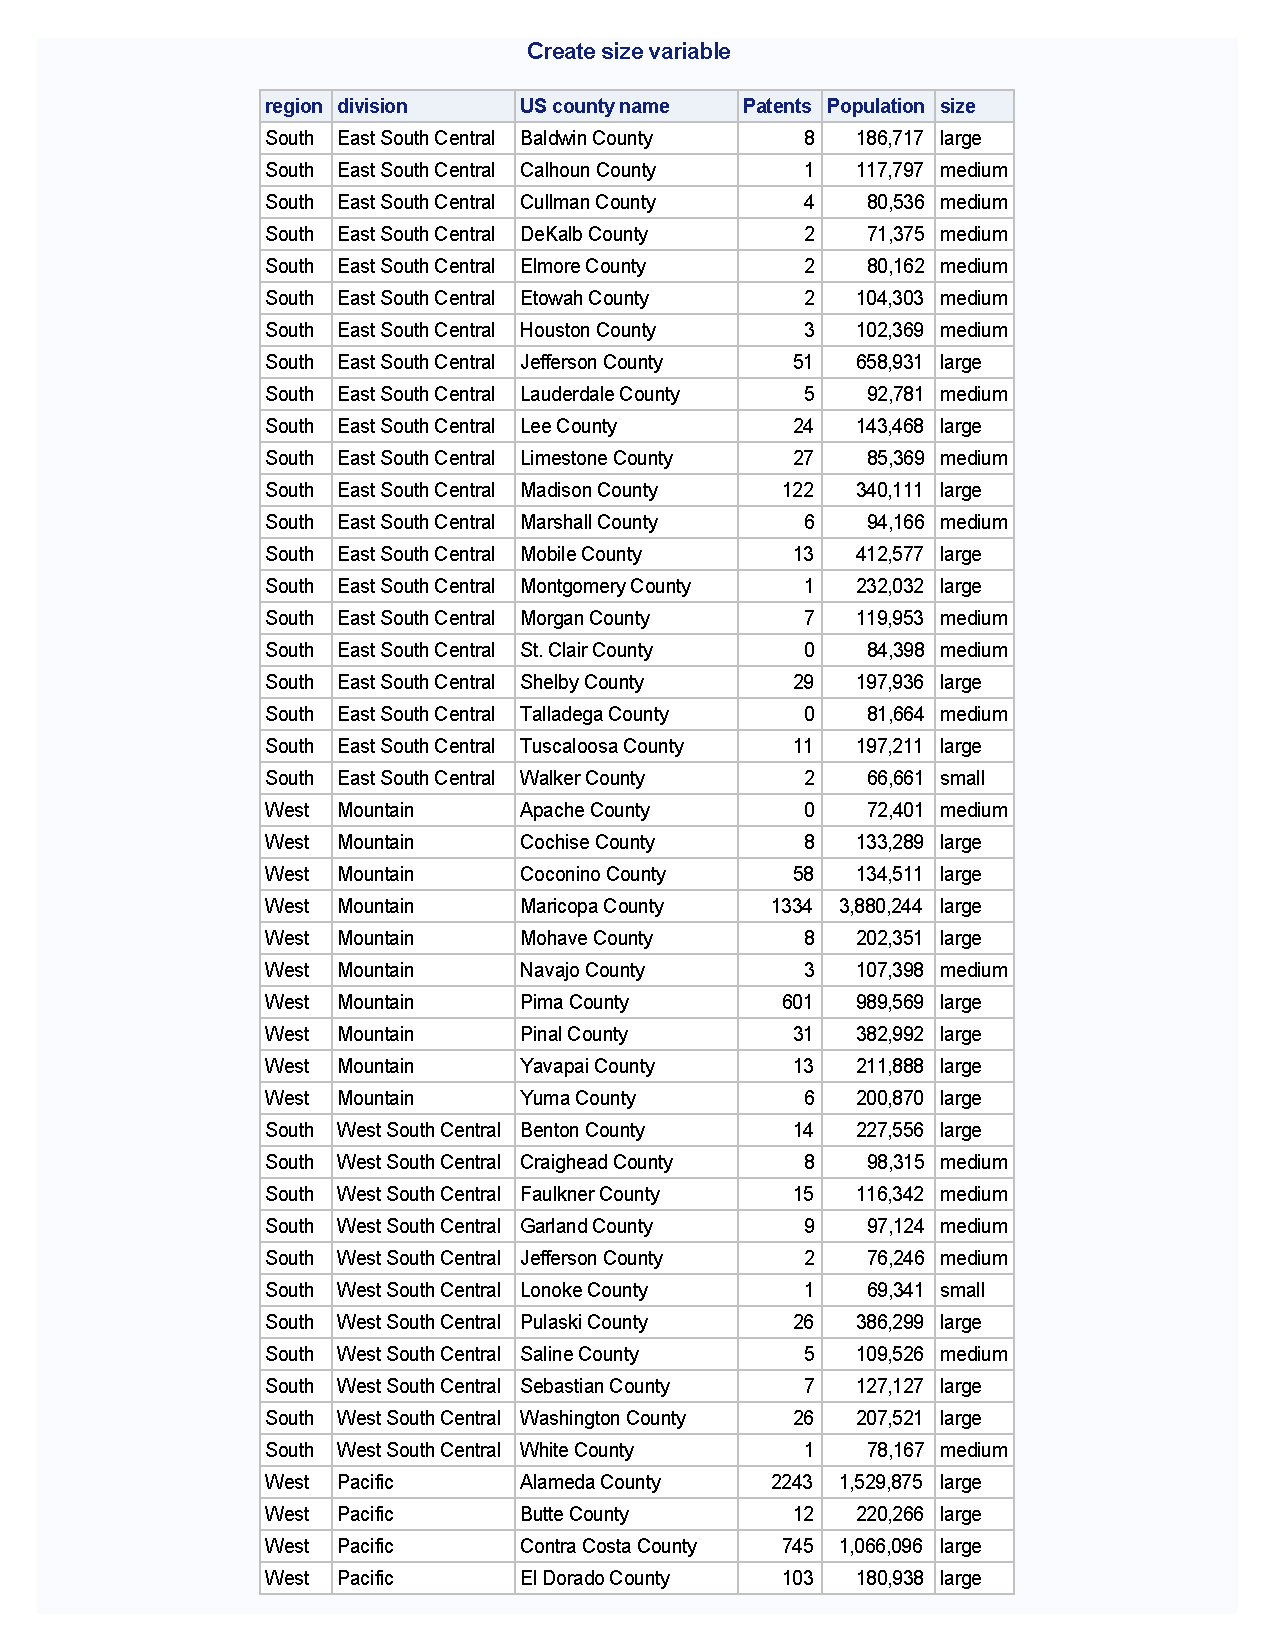
\includegraphics[trim={3.5cm 16cm 3.5cm 1.5cm},clip,width=0.8\textwidth]{L17_case.pdf}
\end{frame}


%===========================================================================================================================
\section[Summarizing data]{Summarizing data}
%===========================================================================================================================
\subsection{}
\begin{frame}
\tableofcontents[currentsection, hideallsubsections]
\end{frame}

\begin{frame}[fragile]
\ft{Getting started}
\bmp{0.68\textwidth}
\begin{code}{.}
PROC SQL;
   SELECT region,
          \textcolor{OrangeRed}{COUNT(county) AS NumCounties}
   FROM patents
   \textcolor{OrangeRed}{GROUP BY region}
   ;
QUIT ;
\end{code}
\emp
\blankcolumn
\bmp{0.38\textwidth}
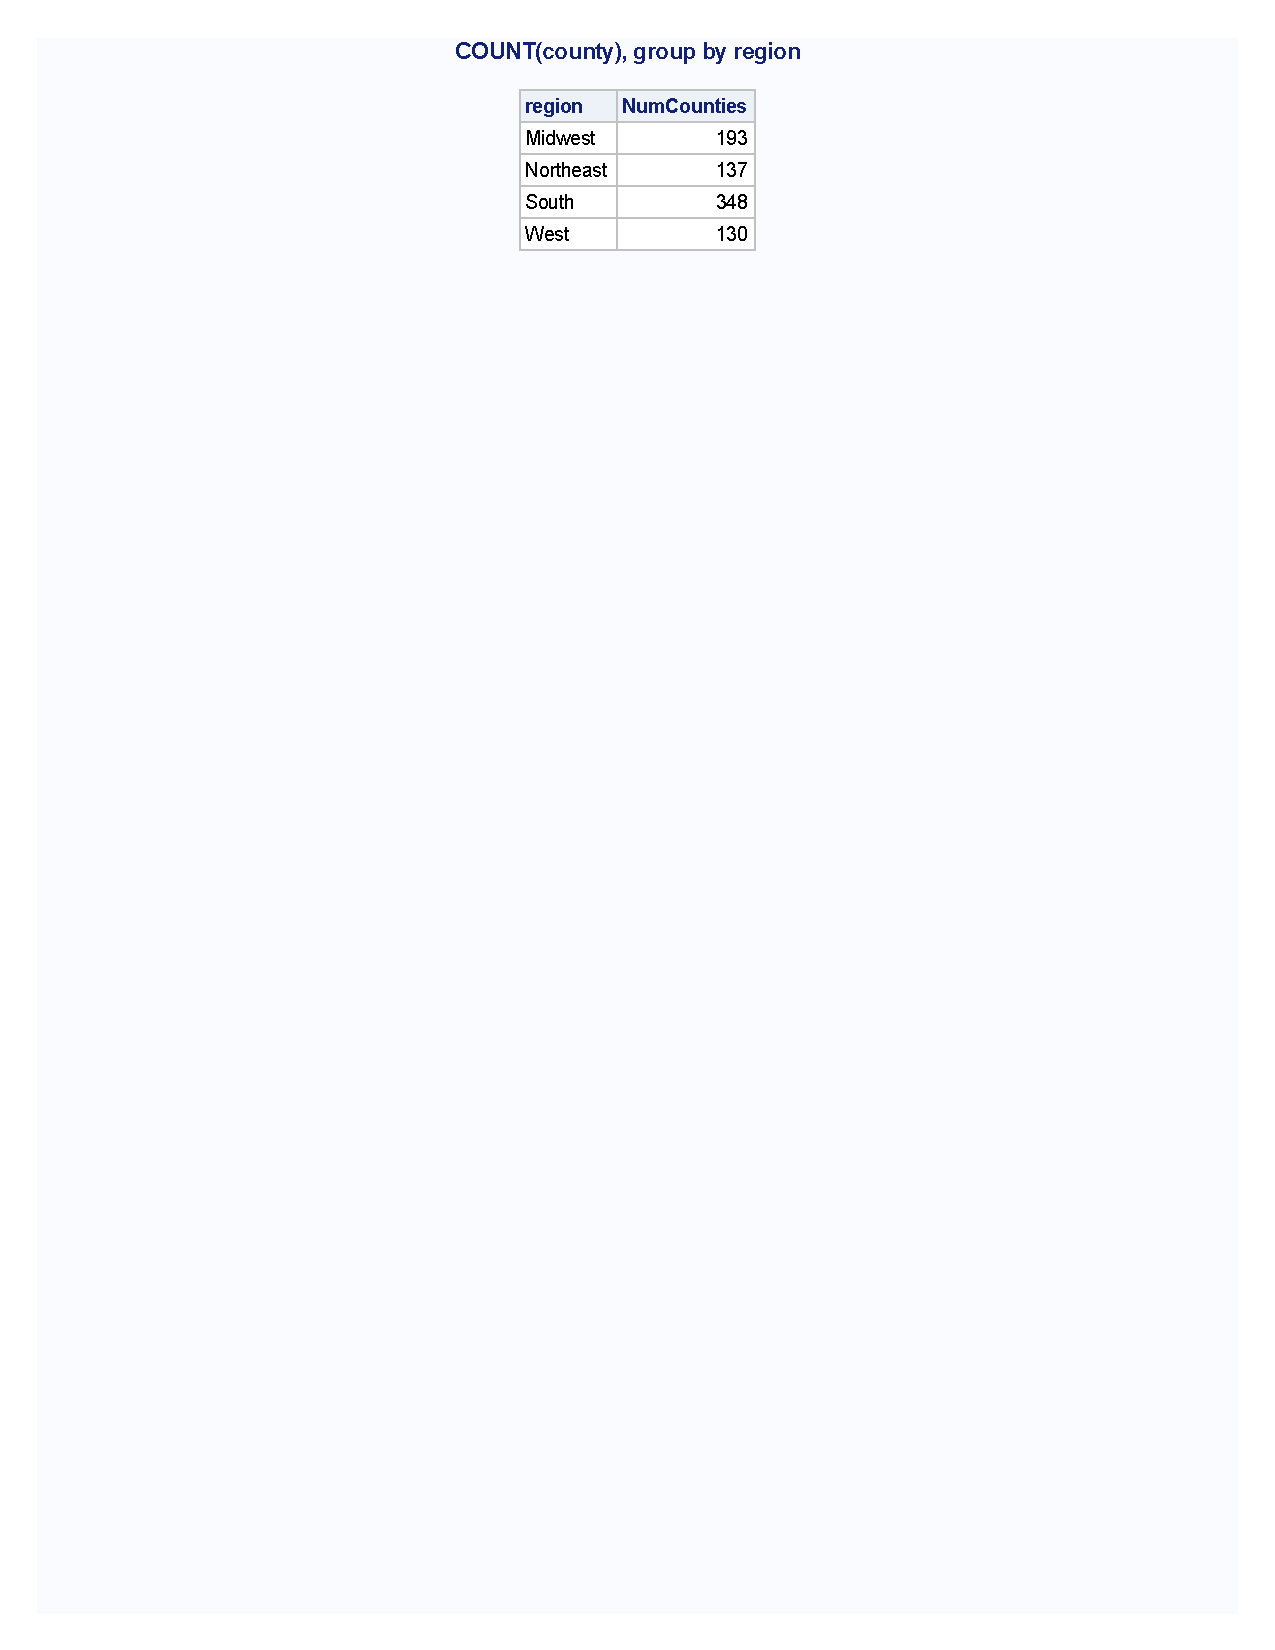
\includegraphics[trim={8.5cm 23cm 8.5cm 1.5cm},clip,width=0.8\textwidth]{L17_count.pdf}
\emp

\vskip5pt
\begin{itemize}
\item Syntax: \fbox{\ttt{\emph{FUNCTION}(\emph{var}) AS \emph{newvar}}}
\item create variable with summary values on \ttt{SELECT} clause
\item indicate how to summarize with \ttt{GROUP BY} clause
\end{itemize}
\end{frame}

\begin{frame}
\ft{Summary functions}
\begin{tabular}{p{4cm} p{3cm} p{3cm}}
COUNT/FREQ/N & SUM & AVG/MEAN \\
MIN & MAX & RANGE \\
STD & VAR & USS \\
CSS & T & NMISS\\
\end{tabular}
\bi
\item[]
\item these functions summarize data over observations
\item think vertical summary, not horizontal
\item so the \ttt{MEAN} function in \ttt{PROC SQL} works like \ttt{PROC MEANS} and \ttb{not} like the \ttt{mean} function in a \ttt{DATA step}
\ei
\end{frame}

\begin{frame}[fragile]
\ft{Counting missing values}
\bmp{0.50\textwidth}
\begin{code}{.}
PROC SQL ;
   SELECT region,
      \textcolor{OrangeRed}{COUNT(asian) AS N1},
      \textcolor{OrangeRed}{NMISS(asian) AS N2}
   FROM patents
   GROUP BY region
   ;
QUIT;
\end{code}
\emp
\bmp{0.05\textwidth} \hspace{0.05in} \emp
\bmp{0.42\textwidth}
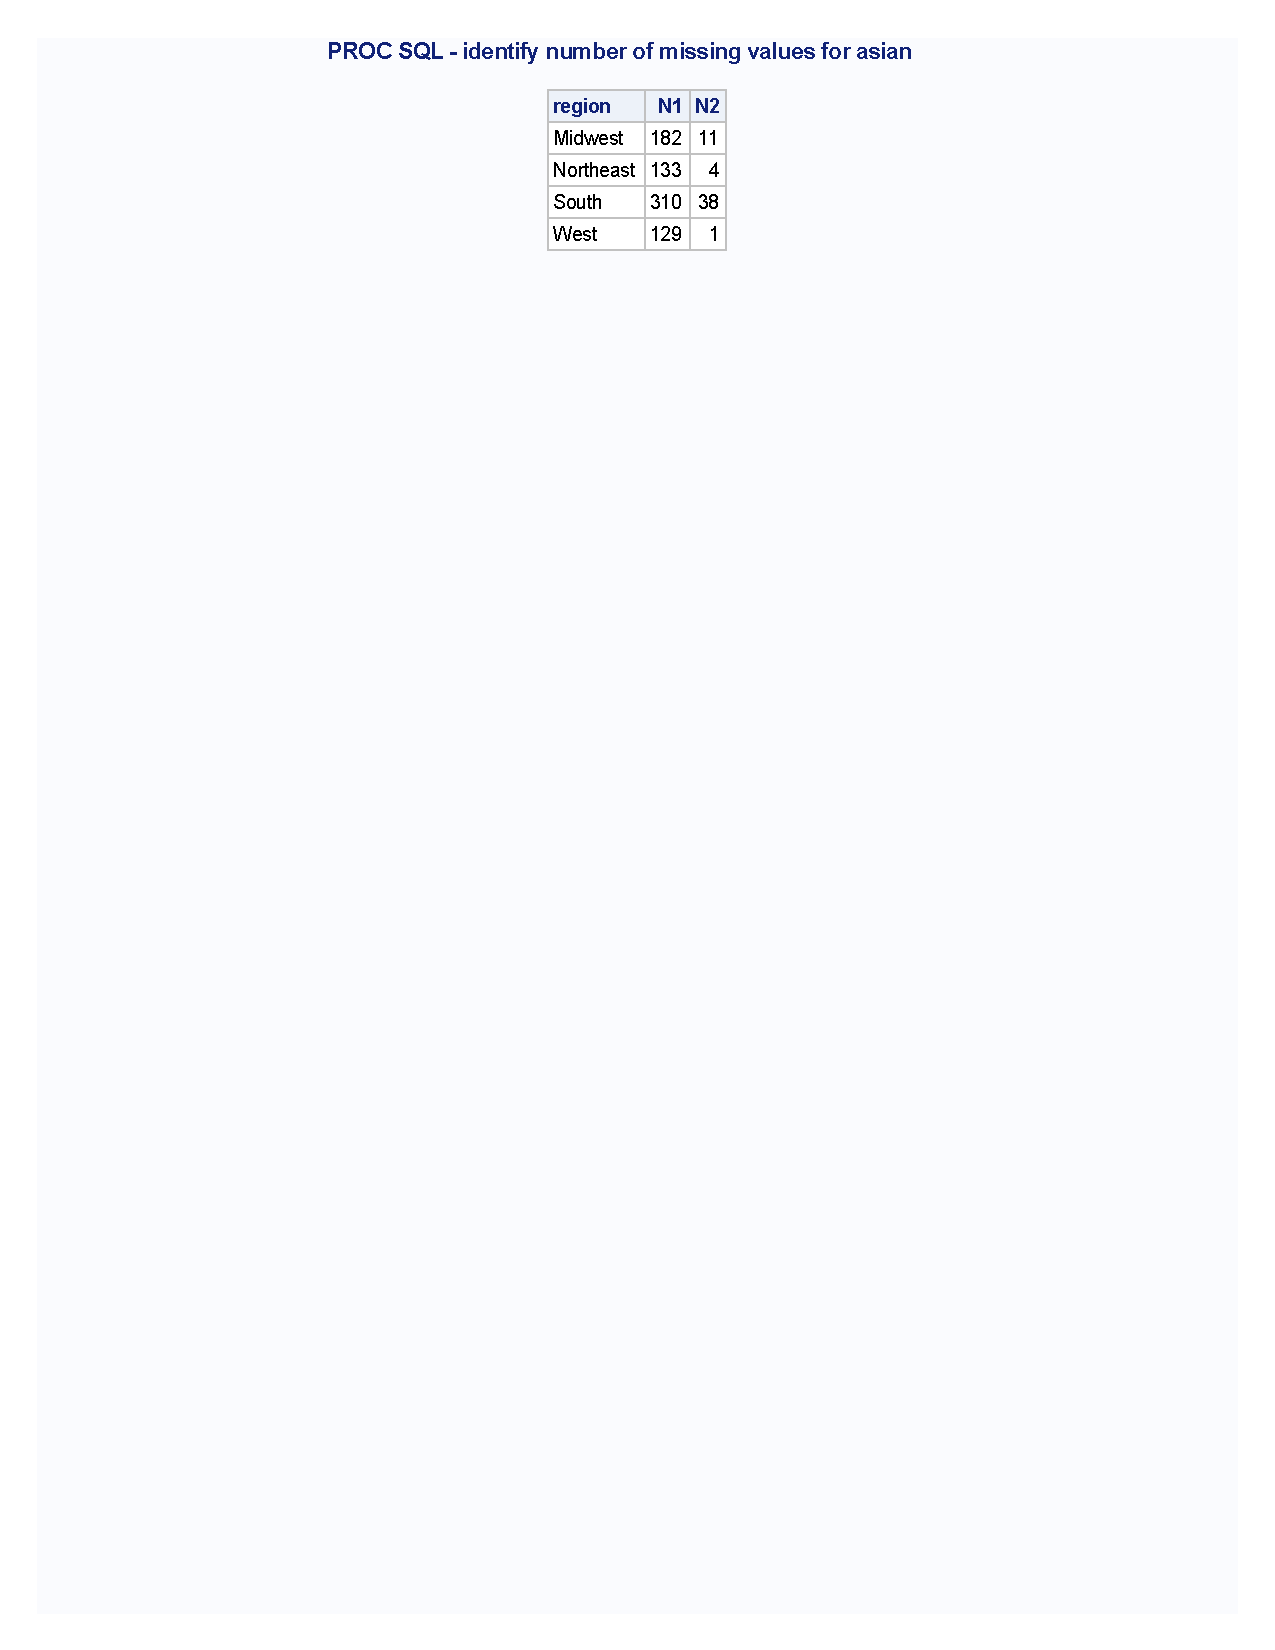
\includegraphics[trim={8.5cm 23cm 8.5cm 1.5cm},clip,width=0.8\textwidth]{L17_count2.pdf}
\emp
\bi
\item[]
\item \ttt{COUNT} returns the number of non-missing observations
\item \ttt{NMISS} returns the number of missing observations
\ei
\end{frame}


\begin{frame}[fragile]
\ft{Discussion}
\hspace*{-0.1in}
\bmp{0.42\textwidth}
\begin{code}{.}
PROC SQL;
   SELECT
      region, \textcolor{OrangeRed}{\fbox{\emph{summary}}}
   FROM patents
   \textcolor{OrangeRed}{GROUP BY region}
   ;
quit;
\end{code}
\emp
%\bmp{0.05\textwidth} \hspace{0.05in} \emp
\bmp{0.70\textwidth}
\bi
\item \ttt{COUNT(county) AS NumCounties}
\item \ttt{COUNT(division) AS NumDivision}
\item \ttt{COUNT(patents) AS NumPatents}
\ei
\emp
\vskip5pt
\begin{clicker}{Assume that there are no missing values in \ttt{county}, \ttt{division}, and \ttt{patents}.  Identify the relationship.}
\begin{enumerate}
\item \ttt{NumDivision} ($<$, $>$, $=$) \ttt{NumCounties}
\item \ttt{NumPatents} ($<$, $>$, $=$) \ttt{NumCounties}
\end{enumerate}
\end{clicker}
\end{frame}

\begin{frame}[fragile]
\ft{Other summary stats}
\hspace*{-0.3in}
\bmp{0.50\textwidth}
\begin{code}{.}
PROC SQL;
   SELECT
      REGION,
      \textcolor{OrangeRed}{COUNT(county) AS N,}
      \textcolor{OrangeRed}{SUM(patents) AS TotP,}
      \textcolor{OrangeRed}{MEAN(patents) AS AveP}
   FROM patents
   GROUP BY region
   ;
QUIT;
\end{code}
\emp
\blankcolumn
\bmp{0.60\textwidth}
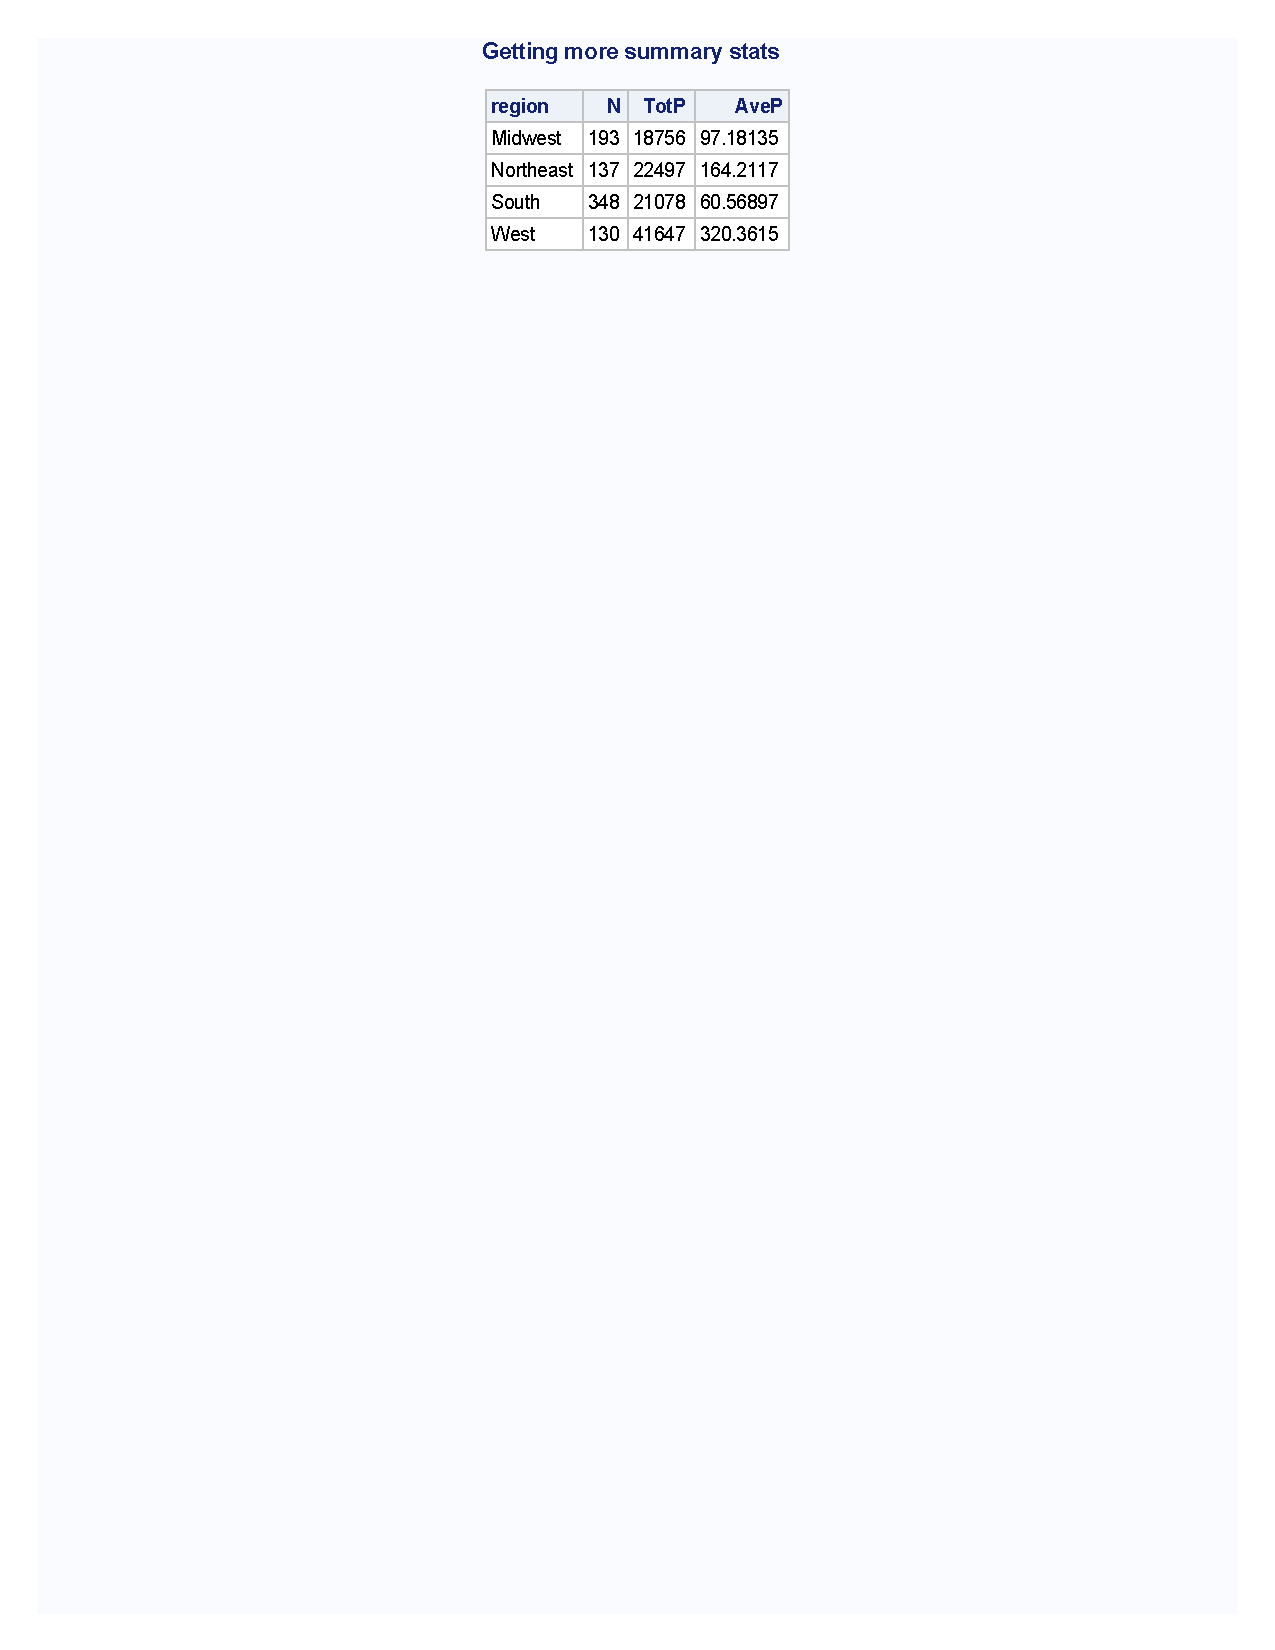
\includegraphics[trim={7.5cm 23cm 7.5cm 1.5cm},clip,width=0.8\textwidth]{L17_stats.pdf}
\emp
\end{frame}

\begin{frame}[fragile]
\ft{Multiple groupings, ex1}
\hspace*{-0.3in}
\bmp{0.50\textwidth}
\begin{code}{.}
PROC SQL ;
   SELECT
      \textcolor{OrangeRed}{region, division,}
      COUNT(county) AS N
   FROM patents
   \textcolor{OrangeRed}{GROUP BY region, division}
   ;
quit;
\end{code}
\emp
\blankcolumn
\bmp{0.60\textwidth}
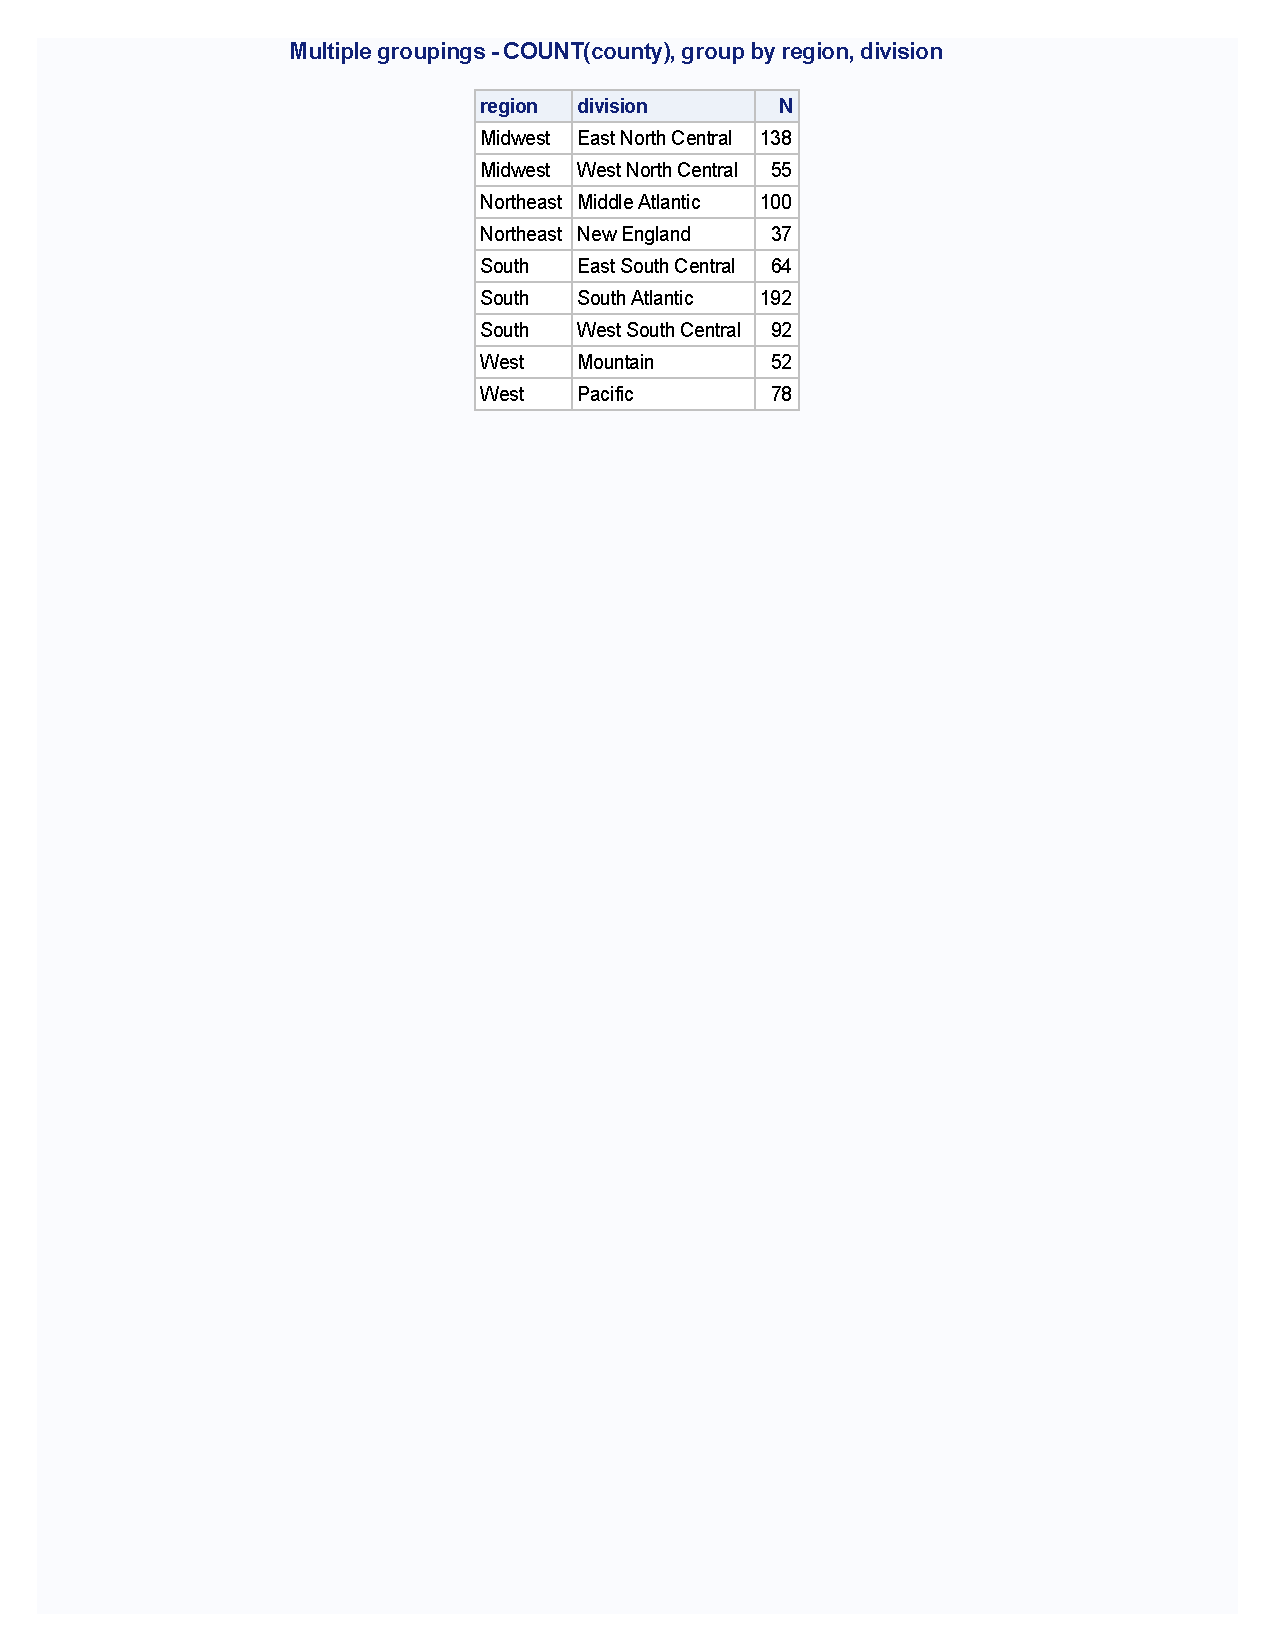
\includegraphics[trim={7.5cm 21cm 7.5cm 1.5cm},clip,width=0.8\textwidth]{L17_multgroup.pdf}
\emp
\bi
\item[]
\item obtain sample size for region/division
\ei
\end{frame}

\begin{frame}[fragile]
\ft{Multiple groupings, ex2}
\hspace*{-0.35in}
\bmp{0.50\textwidth}
\begin{code}{.}
PROC SQL ;
   SELECT
      \textcolor{OrangeRed}{region, edu25,}
      COUNT(county) AS N,
      SUM(patents) AS TotP,
      MEAN(patents) AS AveP
   FROM patents
   \textcolor{OrangeRed}{GROUP BY region, edu25}
   ;
QUIT;
\end{code}
\emp
\blankcolumn
\bmp{0.60\textwidth}
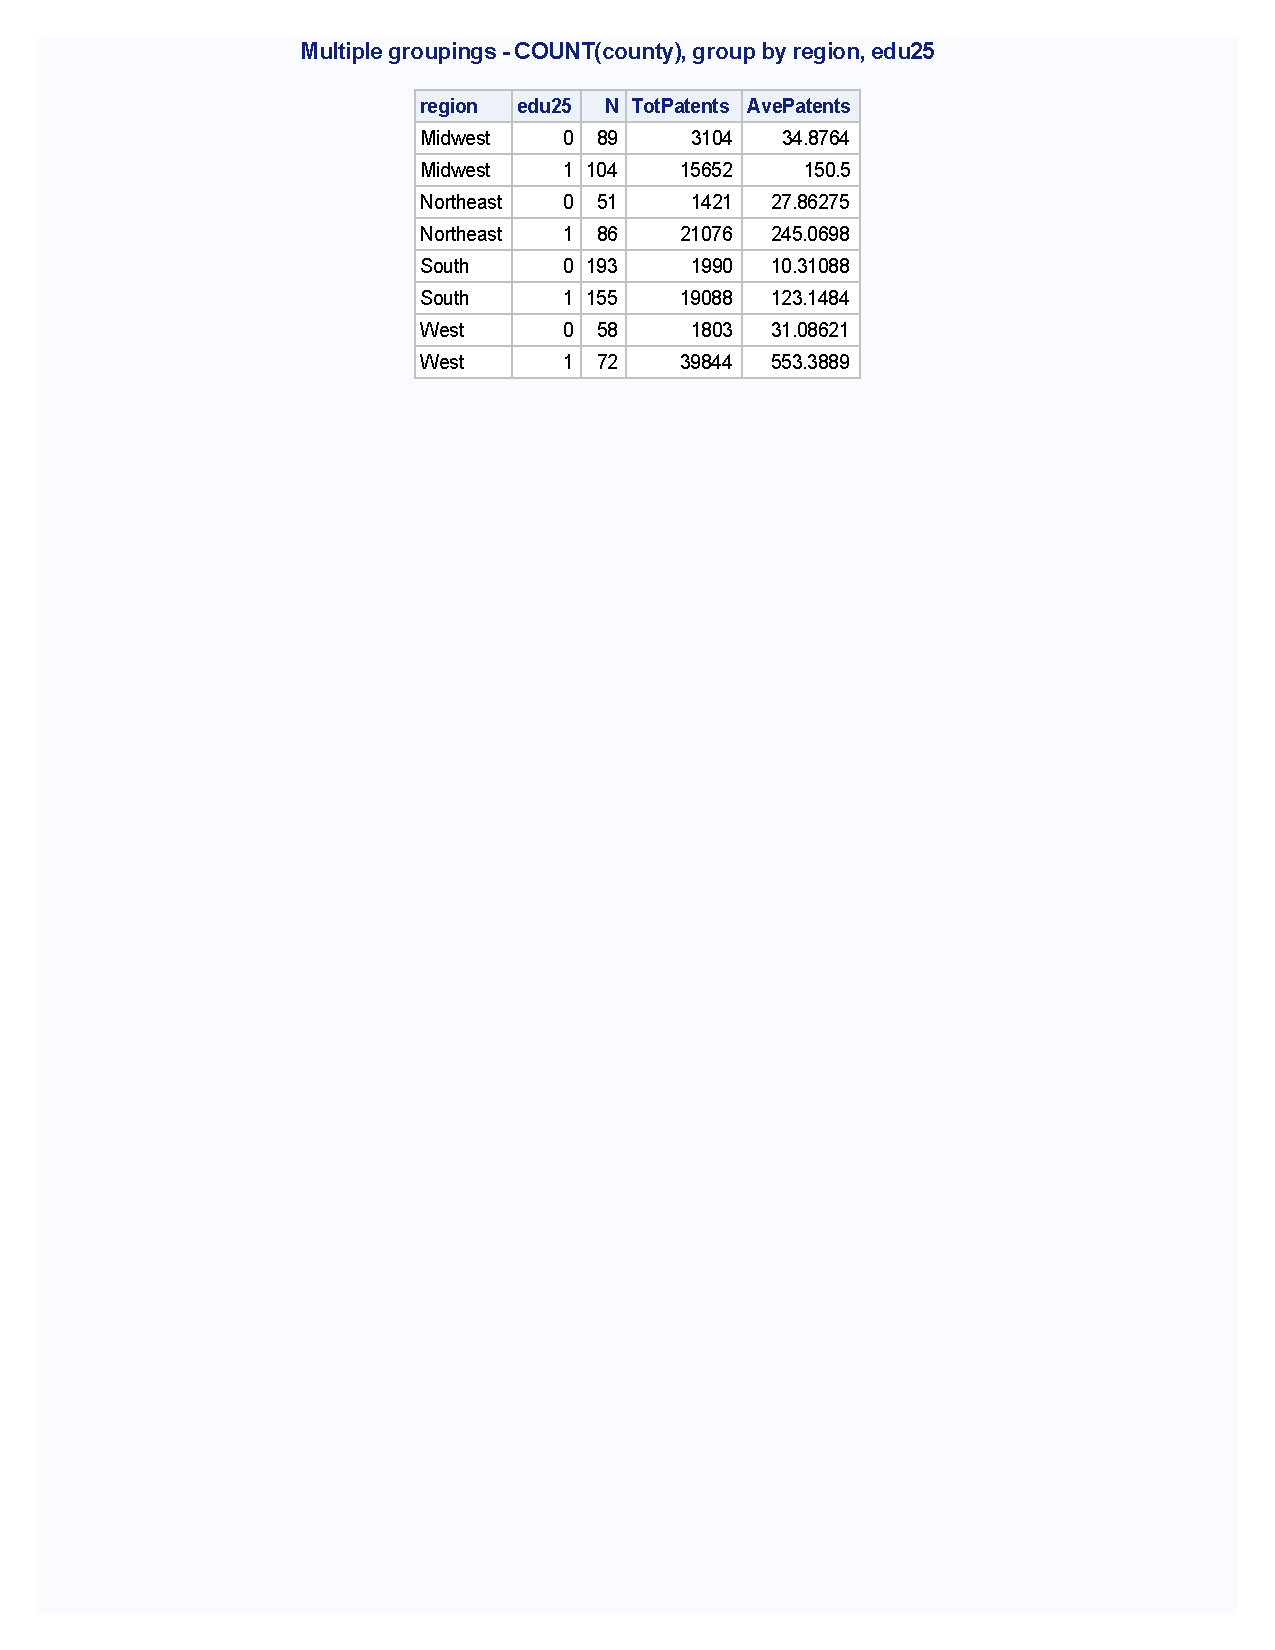
\includegraphics[trim={6.5cm 21cm 6.5cm 1.5cm},clip,width=1.0\textwidth]{L17_multgroup2.pdf}
\emp
\bi
\item[]
\item obtain summary statistics for region/edu25
\ei
\end{frame}

%===========================================================================================================================
\section[More]{More}
%===========================================================================================================================
\subsection{}
\begin{frame}
\tableofcontents[currentsection, hideallsubsections]
\end{frame}

\begin{frame}[fragile]
\ft{Sorting}
\bmp{0.60\textwidth}
\begin{code}{.}
PROC SQL;
   SELECT county, patents
   FROM patents
   WHERE state="WEST VIRGINIA"
   \textcolor{OrangeRed}{ORDER BY patents}
   ;
QUIT;
\end{code}
\emp
\blankcolumn
\bmp{0.35\textwidth}
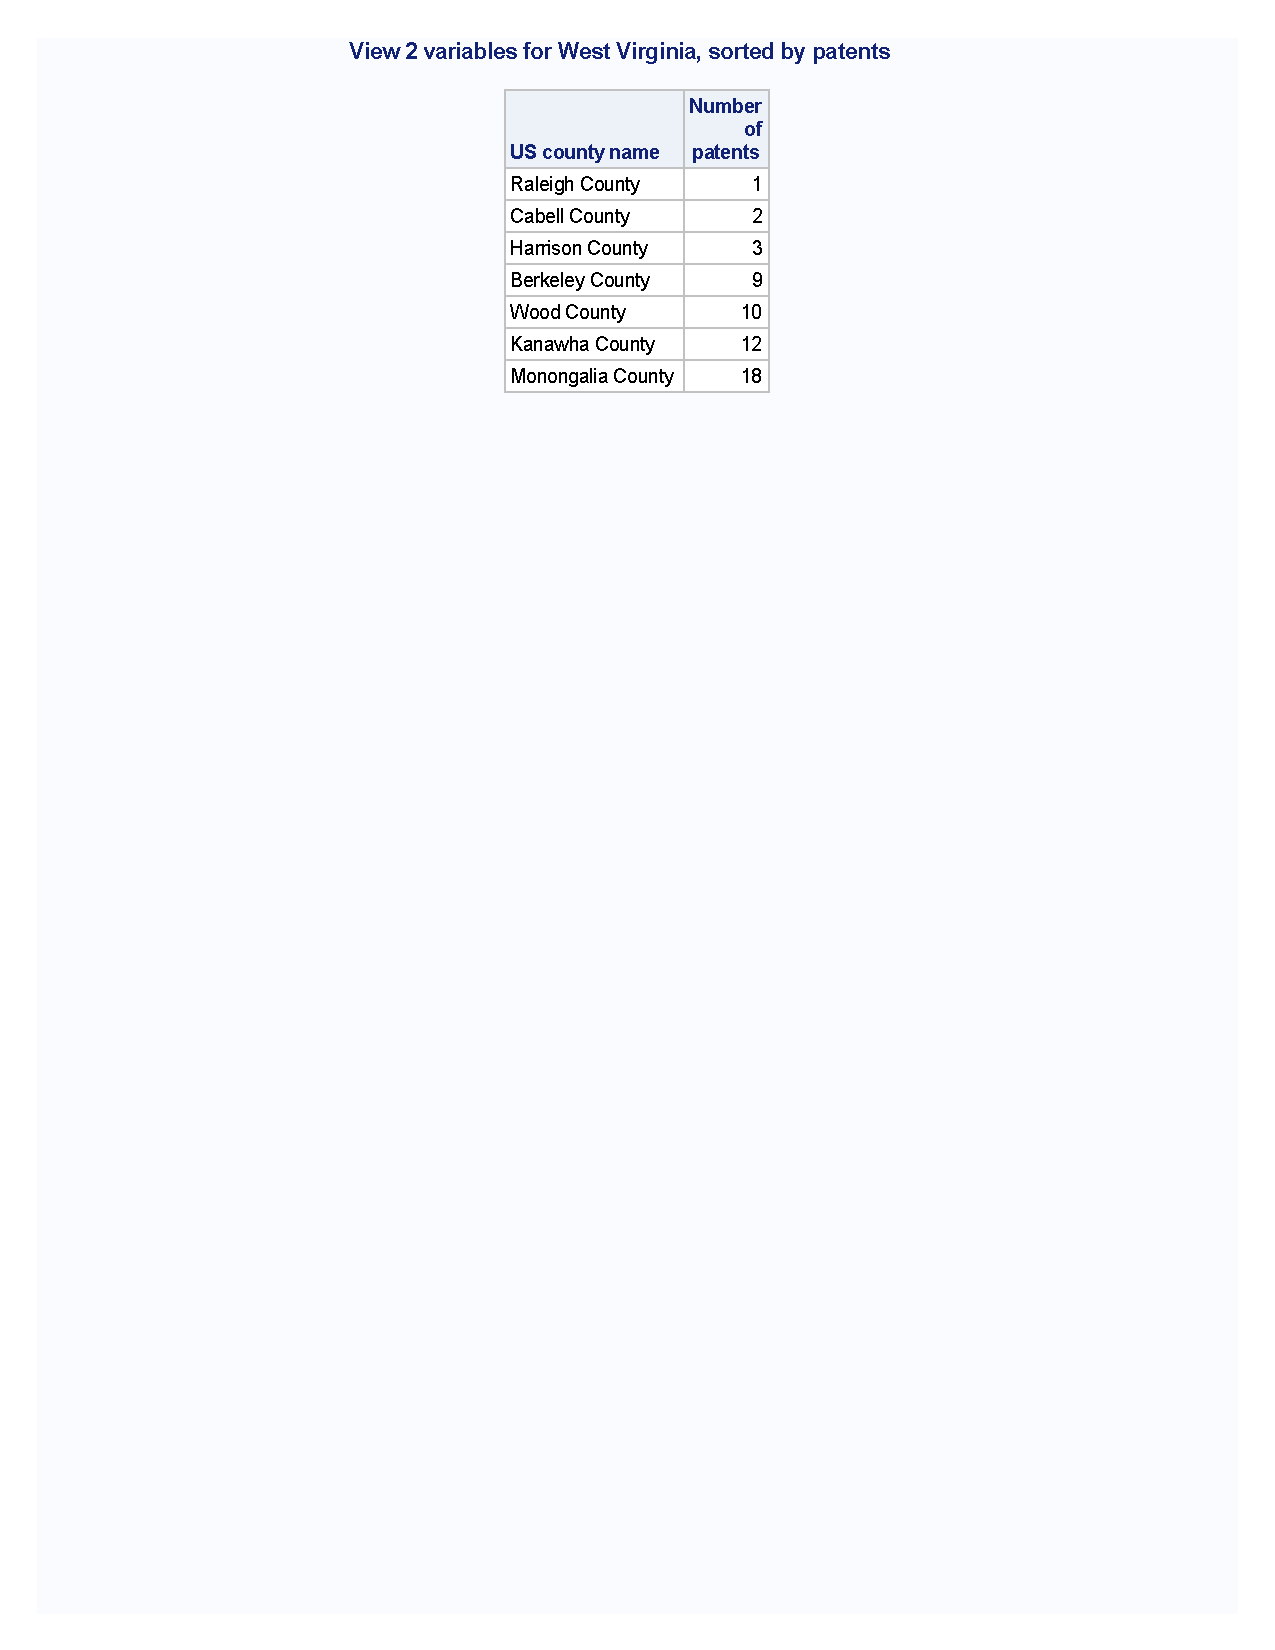
\includegraphics[trim={8cm 21cm 8cm 1.5cm},clip,width=1.0\textwidth]{L17_order.pdf}
\emp
\bi
\item[]
\item can sort by character or numeric variables
\item can sort by multiple variables, separated by comma
\item sorting variable doesn't need to be in \ttt{select} clause
\ei
\end{frame}

\begin{frame}[fragile]
\ft{Creating a data set}
\bmp{0.75\textwidth}
\begin{code}{.}
PROC SQL ;
   \textcolor{OrangeRed}{CREATE TABLE wv AS}
   SELECT region, division, county, patents
   FROM patents
   WHERE state="WEST VIRGINIA"
   ORDER BY patents
   ;
QUIT;

PROC PRINT DATA = \textcolor{OrangeRed}{wv} ;
RUN ;
\end{code}
\emp
\bi
\item[]
\item Syntax: \fbox{\ttt{CREATE TABLE \emph{datasetname} AS}}
\item no output generated from PROC SQL
\ei
\end{frame}

\begin{frame}[fragile]
\ft{Using DISTINCT, example 1}
\bmp{0.60\textwidth}
\begin{code}{.}
PROC SQL;
  SELECT region,
    COUNT(county) AS N1,
    COUNT(\textcolor{OrangeRed}{DISTINCT} county) AS N2
  FROM patents
  GROUP BY region
  ;
QUIT;
\end{code}
\emp
\blankcolumn
\bmp{0.35\textwidth}
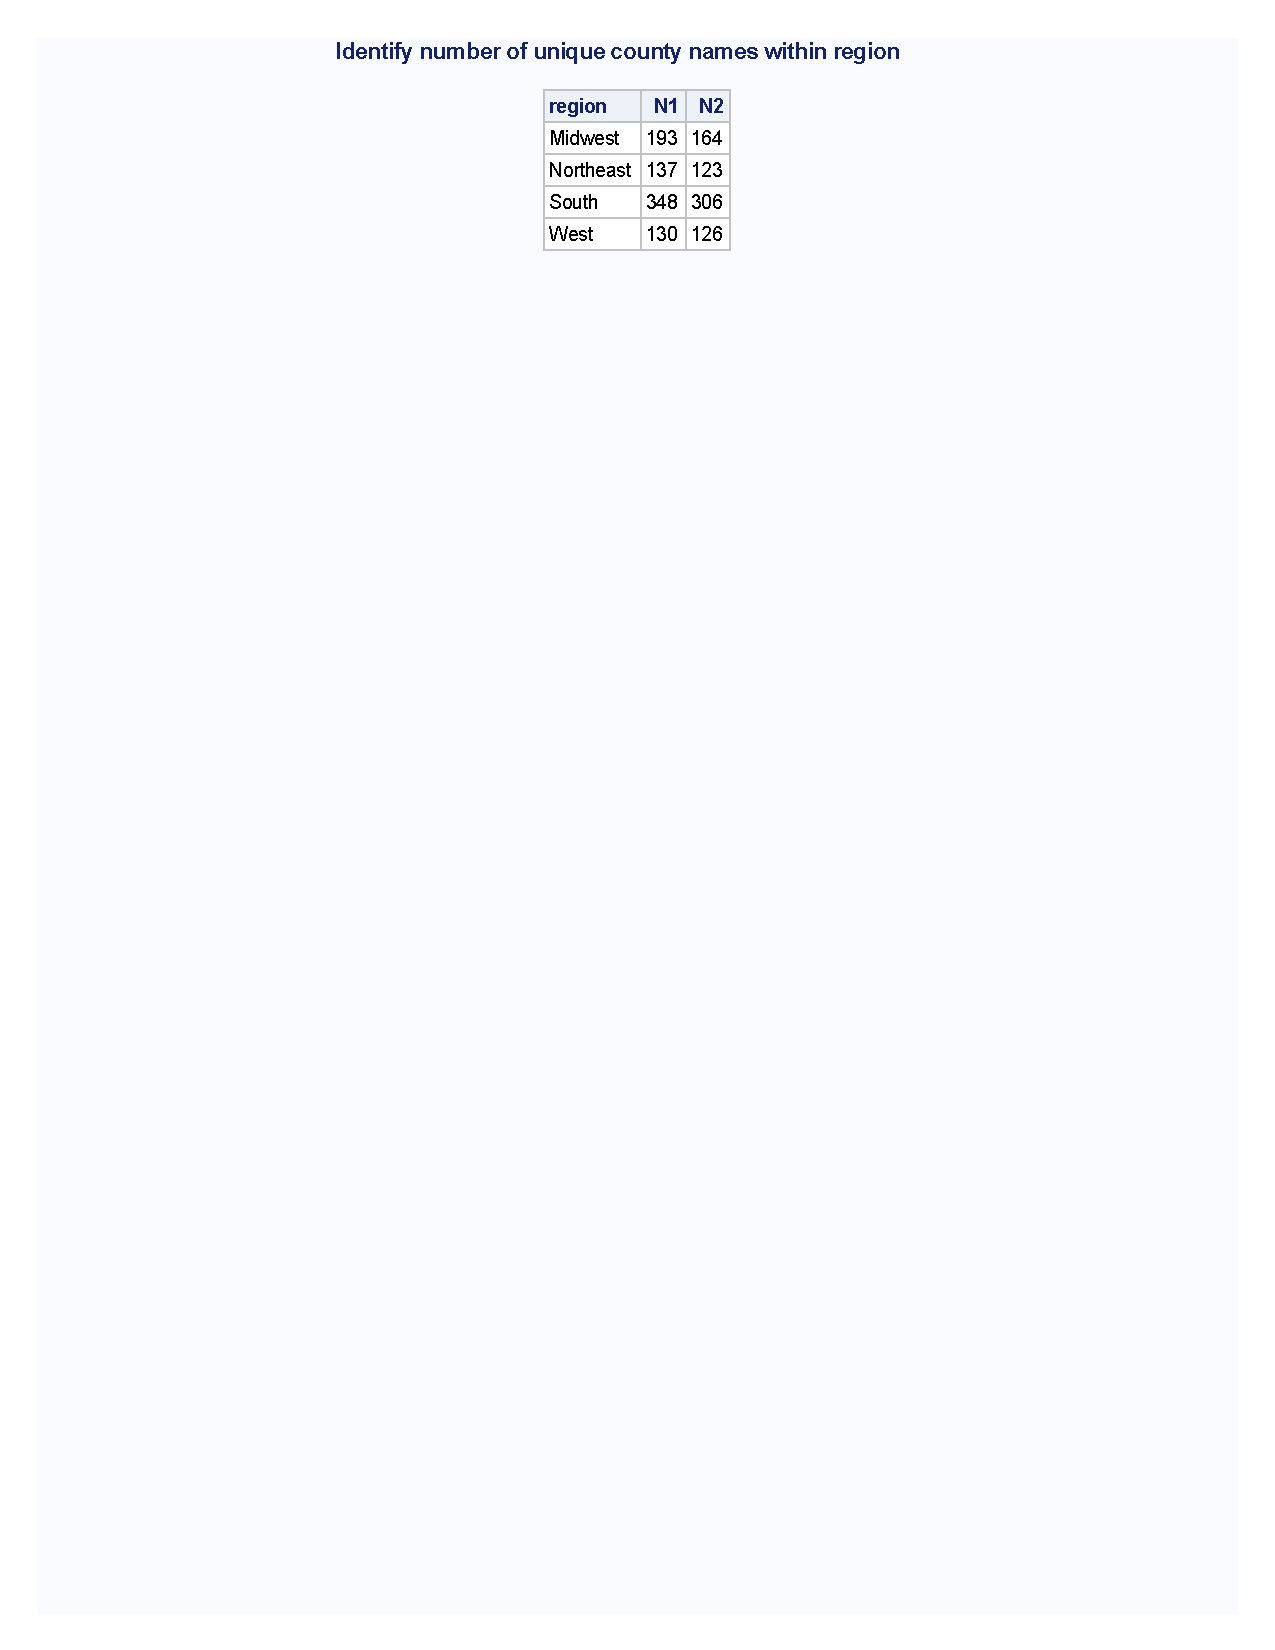
\includegraphics[trim={8cm 23cm 8cm 1.5cm},clip,width=1.0\textwidth]{L17_distinct1.pdf}
\emp
\bi
\item[]
\item \ttt{N1} is the total number of counties in each region
\item \ttt{N2} is the number of unique county names in each region
\ei
\end{frame}

\begin{frame}[fragile]
\ft{Using DISTINCT, example 2}
\bmp{0.60\textwidth}
\begin{code}{.}
PROC SQL ;
   SELECT \textcolor{OrangeRed}{DISTINCT} county
   FROM patents
   WHERE region="Midwest"
   ORDER BY county
   ;
QUIT;
\end{code}
\emp
\blankcolumn
\bmp{0.35\textwidth}
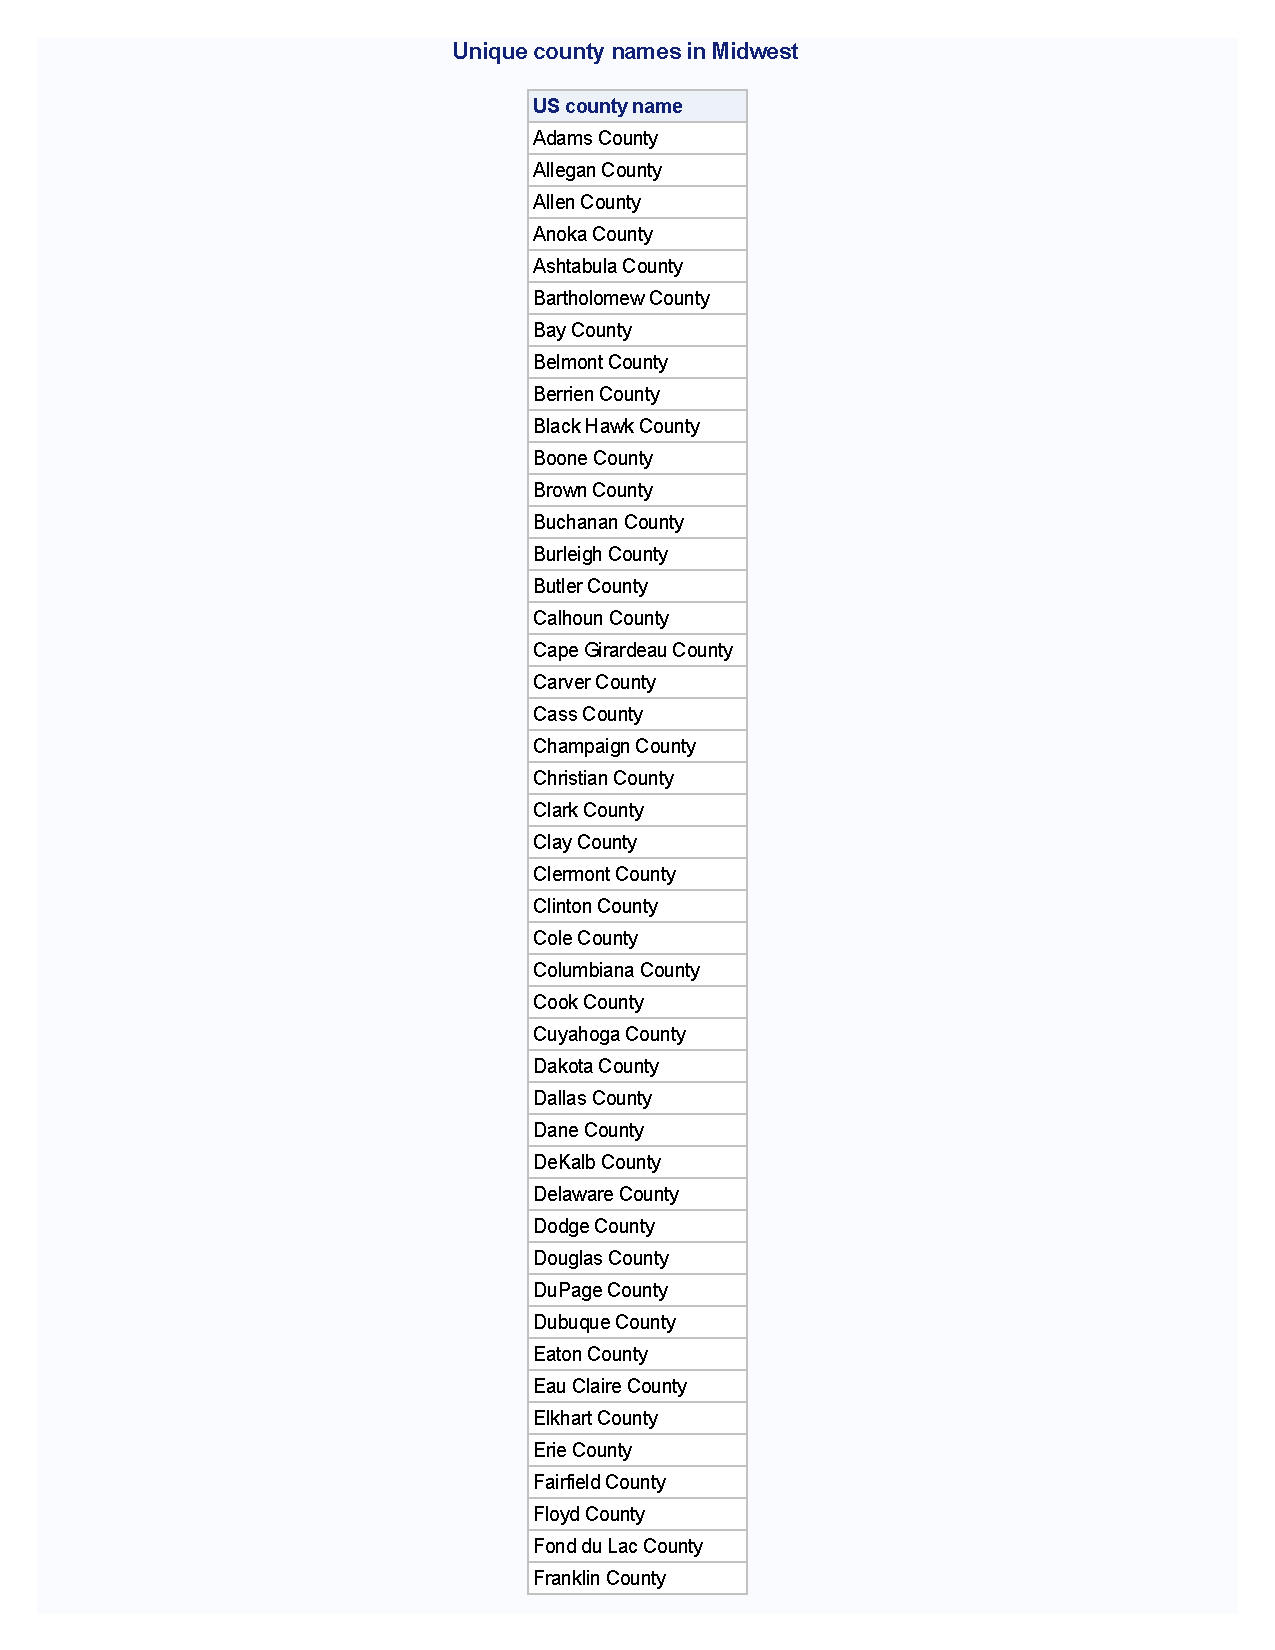
\includegraphics[trim={8cm 18cm 8cm 1.5cm},clip,width=1.0\textwidth]{L17_distinct2.pdf}
\emp
\bi
\item[]
\item prints unique county names in Midwest
\ei
\end{frame}

%\begin{frame}[fragile]
%\ft{Sub query}
%\end{frame}

\begin{frame}[fragile]
\ft{Joins (combining data)}
\begin{tabular}{p{4cm} cc}
\hline
Feature & \ttt{PROC SQL} & \ttt{DATA} step merging \\
\hline \hline
Requires sorted data sets & \rx & \gc \\
& & \\
Requires same name for identifying variable  & \rx & \gc \\
& & \\
Can handle many to many relationship   & \gc & \rx \\
\hline
\end{tabular}
\vskip10pt
\url{http://www.listendata.com/2014/06/proc-sql-merging.html}
\end{frame}





\end{document} 